\chapter{Robot}

Let me introduce to the topic of my PhD work at \acrfull{sk}.

\todo[inline]{TODO: complete chapter}

\section{Thesis Structure}
The diagram in \autoref{fig:thesis-structure} illustrates the flow of information through the structure of the thesis.

\begin{figure}[htb!]
\centering 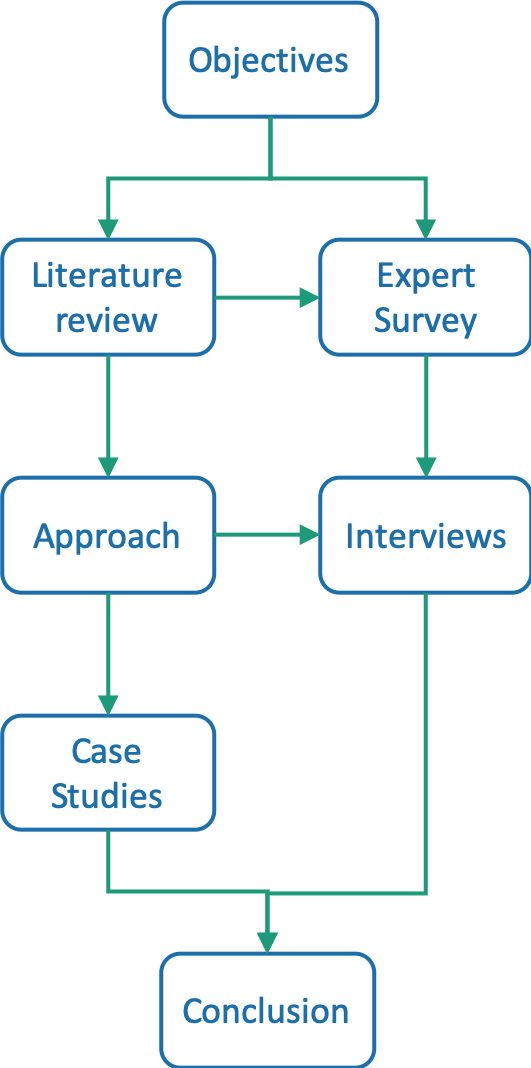
\includegraphics[width=0.5\textwidth]{graphics/thesis-structure}
\caption{Thesis structure}
\label{fig:thesis-structure}
\end{figure}

\begin{description}
    \item[\Autoref{cap:background} - Background]
Here's the literature review.

    \item[\Autoref{cap:thesis_objectives} - Thesis Objectives]
We define the objectives of our work.

...

    \item[\Autoref{cap:conclusion} - Conclusion]
In the last chapter, we discuss our results obtained ...

%%%%%%%%%%%%%%%%%%%%%%%%%%%%%%%%%%%%%%%%%%%%%%

Let us describe the main design decisions behind the proposed autonomous platform. First of all the target environment should be considered. It is a greenhouse 300 x 400 m where several hundred lines of tomatoes are growing. In the middle of the greenhouse there is concrete road elevated above the main floor. The tomatoes are growing in alliances perpendicular to this center LA. In order for the robot to be true autonomous it is supposed to have two modes of commotion specifically on the concrete floor and on the rails. While the movement on the rails can be implemented in a straightforward manner, they design decision for the concrete is not as simple. On the one hand with the number of actuators necessary should be kept at minimum. Moreover, any kind of complicated real system will be prone to the elements from the surrounding. The environment in the greenhouse is humid, and there could be grains of sand, dust, or even small puddles of water here and there. On the other hand, the width of the concrete road is approximately 3 m. It allows for convenient to side walking for the personnel and manual movement of the machinery. However, the algorithms that control freely moving, Robert have to be capable of executing, sharp terms and obstacle avoidance maneuvers. After rigorous consideration and literature review McCannon wheels based system was designed. It is much more mechanically complicated than the regular car like platform with only the front wheels steering, but it allows for the Omni directional motion, as well as turning on the spot. Four wheels were placed at the corners of the robot, which should remain the same during all the modifications. An important factor is this smoothness in the uniformity of the concrete surface that cannot be guaranteed in the unknown environment. Thus an individual suspension module for each of the wheels was designed. Modern greenhouses are standardized, meaning that they have the rails at a specified distance from each other. So the geometrical configuration of the robot was derived from that. The first version of the robot was designed and assembled, which was followed by the real test in a greenhouse during the tomato production. During the testing, it has become clear that despite the specifications, unknown and unpredictable circumstances can appear. One of the main ones was that despite the robot properly feeding in the in between the lines of the tomatoes it was at times, touching the tomato plant parts that were hanging lower than they should be. The integration of an agricultural robot should be performed as smooth as possible, meaning the non-invasive manner and keeping the greenhouse modifications to the bare minimum as well as the workflow there. Thus a decision was made to reduce the width of the robot by integration, the activators inside the wheel itself. With such a modification, the robot has become even more compact minimizing the probability of the contact between it and the plant. The road wheels and the rail wheels are mounted coax keeping the number of the activator is necessary down to only four. The motors that are used in the last third version of the robot are normally used in electric bikes. They are protected from the humidity and dust and are capable of functioning in a wide range of external conditions, including temperature. Moreover, with the current mass of the robot, the perspective velocity and the limited acceleration, they are used under very moderate load, assuring their longevity and reducing the need for maintenance. During the design of the last version of the wheel modules, a model of mechanical wheels that was found convenient, was reproduced using more rigid type of steel. The wheels from the second version of the Robert broke during the testing, making it necessary to develop a more sturdy version. All in all the last version of the wheel modules can be used on the scope of the agriculture, agricultural applications. They could be mounted to an object with a few modifications, only the mounting surfaces and the necessary wiring. The control boards of the wheels were chosen so that they can carry much heavier loads in terms of the current then the ones that typically appear in the robot. Regarding the main hall of the robot, it is manufactured from the aluminum tubes with square cross-section and planer aluminum elements. In the first version of the robot composite materials were used to manufacture the planer elements. Later they were changed to aluminum. It is heavier, but it provides rigidity to the structure of the robot. Moreover, it lifts the burden of active cooling of the interior of the robot by having a surface area of approximately 2 m². Regarding the electrical supply of the Robert lithium batteries were chosen with high energy density, and the voltage that can that the motors can work with without a converter. Six batteries approximately 5 kg each were replaced in the exterior module of the robot. Thus the internal space can be used to accommodate the computer and other equipment. The perspective power consumption of 500 W can be sustained for 12 hours. In order to assure smooth integration of all the equipment to the robot and DCAC converter was installed on board providing 220 V for all the devices, allowing them to be powered by their default power converters. While this solution is excessive in terms of the power consumption, it makes the integration of novel modules easier. The devices on board include the main computing module, which is a laptop with a discrete GPU wi-Fi router, a set of cameras, a power converter in the charger. The charger was chosen, such that it can charge all the batteries in three hours and can be controlled with our S4 185 protocol. This makes it possible, not only to perform the monitoring autonomously, but also charge autonomously. Wi-Fi router is installed on board in order for the robot to be capable of providing its own wireless network for the convenience of the user. While the greenhouses are often highly automated, they are also often located in remote places that lack sufficient coverage of the Internet providers. Moreover, it could be expensive to provide a wireless network of flow literacy and high bandwidth for all the greenhouse. This was one of the reasons why all the computations are performed on board. The second reason is that with instant on the board computations the result could be obtained instantly. Alternatively, an external server could be installed, but such a solution will require a high band with wireless network, capable of streaming up to six full HD videos simultaneous. With the current developments in the field of mobile computing devices, it is possible to perform the inference of modern neural networks and other algorithms to process data on the board in real time. With the speed of the robot that is acceptable from the safety standpoint and the computational capabilities of an integrated, not integrated discrete GPU the problems of disease, identification, and tomato volume estimation can be solved in real time as the robot drives along the line of tomatoes. The software on Robert is pretty standard in terms of the framework and tools. To 20.0 was used as well as open CV by torch by 3-D Python syphilis plus Ross two. The motor drivers were programmed in C.

robot:
- mechanical frame
- wheels
- electrical subsystem (batteries, motors)
- masts
- software
- cameras



\end{description}

